\newpage
\flushleft
\section*{{Appendix A - 2D Enclosed Flow Results}} 
\label{sec: appendix_a}
\addcontentsline{toc}{section}{Appendix A - 2D Enclosed Flow Results}


\begin{figure}[!ht]
    \noindent\makebox[\textwidth]{
    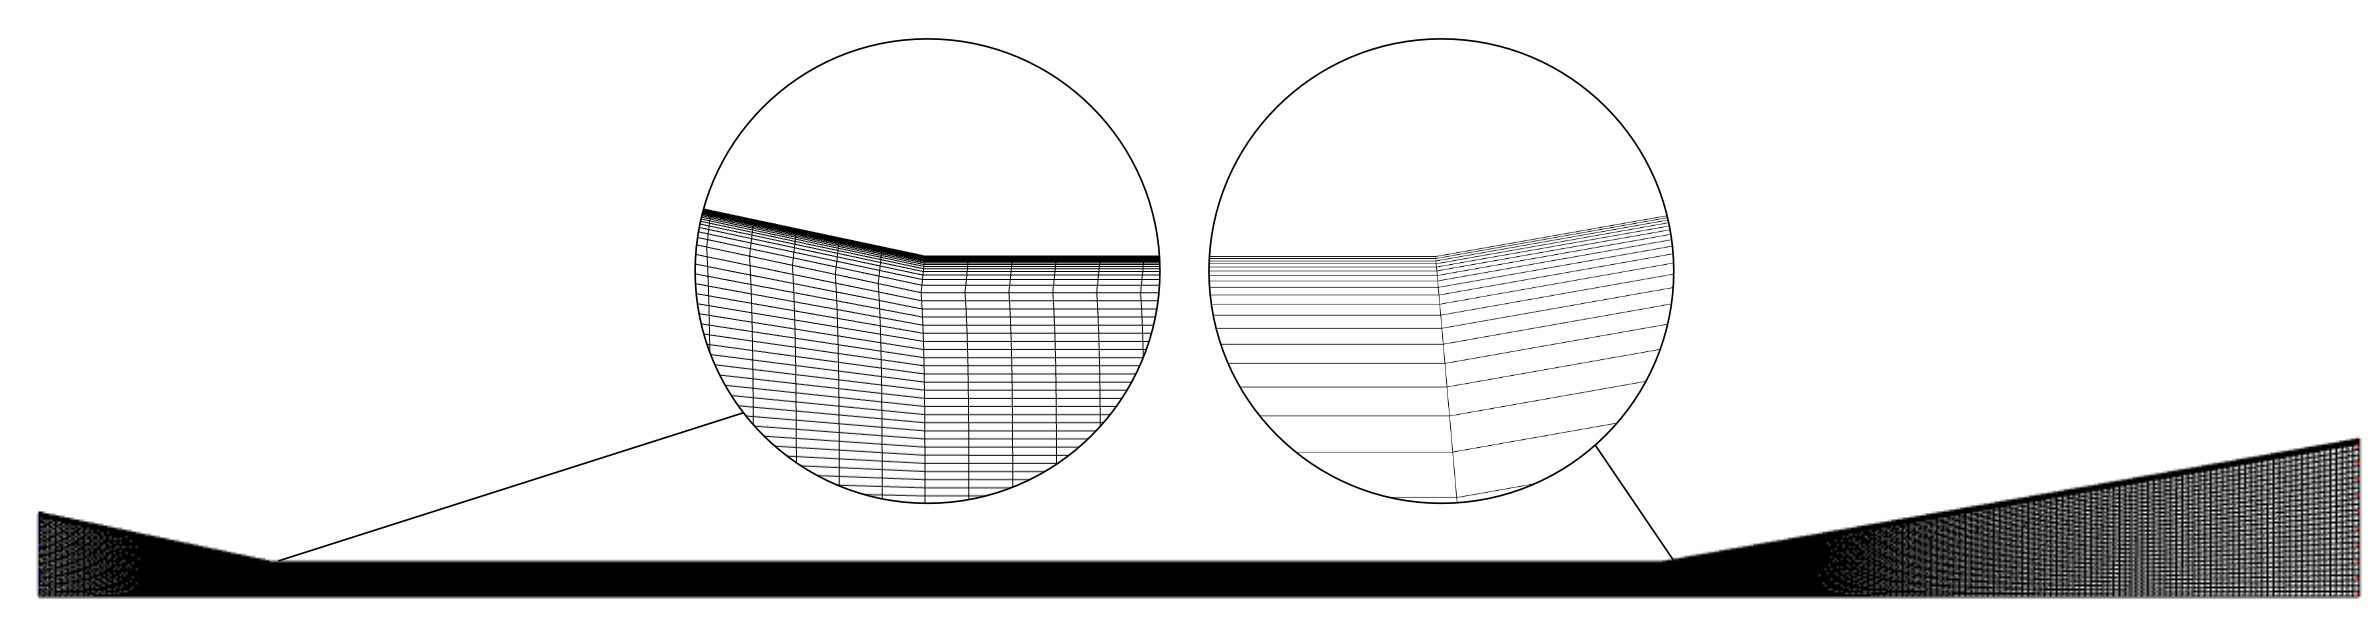
\includegraphics[width=1\textwidth]{Figures/2D_EN/2D_EN_MESH_COMPLETE.png}}
    \caption{2D Enclosed Flow Mesh Consist of Quadrilateral Mesh with 20 Inflation Layer $y^+$=1 Generated} 
    \label{fig:2D_EN_MESH}
\end{figure}

\begin{center}
  \begin{figure}[!ht]
    \noindent\makebox[\textwidth]{
    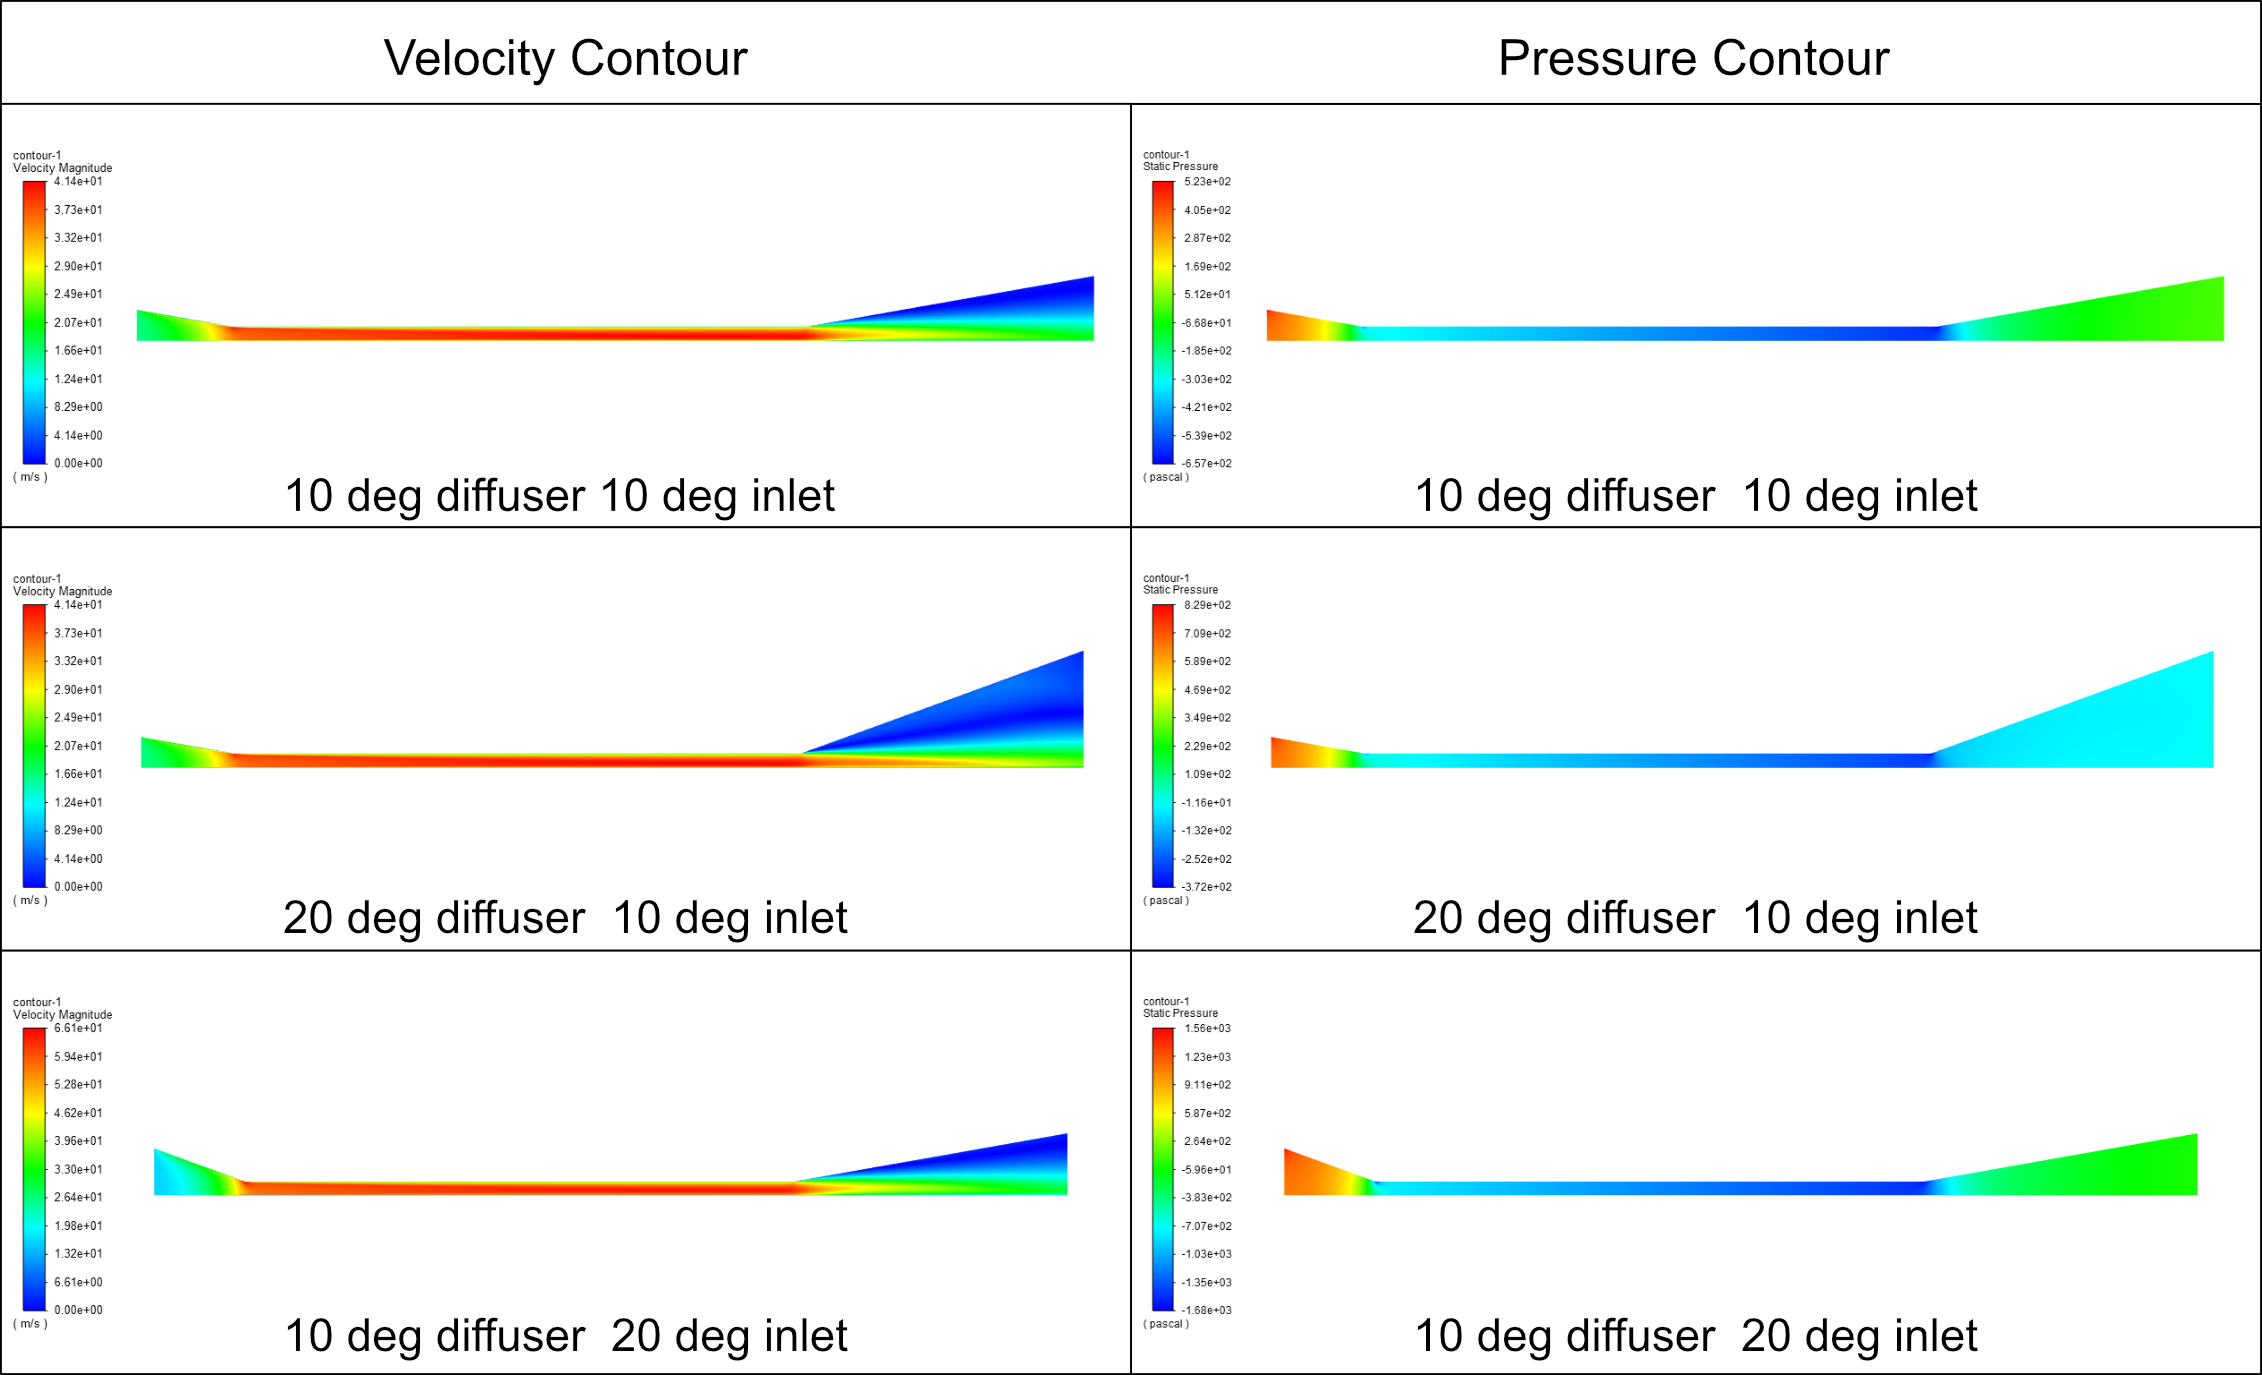
\includegraphics[width=1.1\textwidth]{Figures/2D_EN/COMPILE_APPENDIX_A_PRESSVELO.png}}
    \caption{Velocity (left) and (right) Pressure Contour of The Undertray In Three States: Baseline (top), Maximum Diffuser Angle (middle), and Maximum Inlet Angle (bottom).}
    \label{fig:compile_2D_EN_pressure_velocity}
\end{figure}


\begin{figure}
    \noindent\makebox[\textwidth]{
    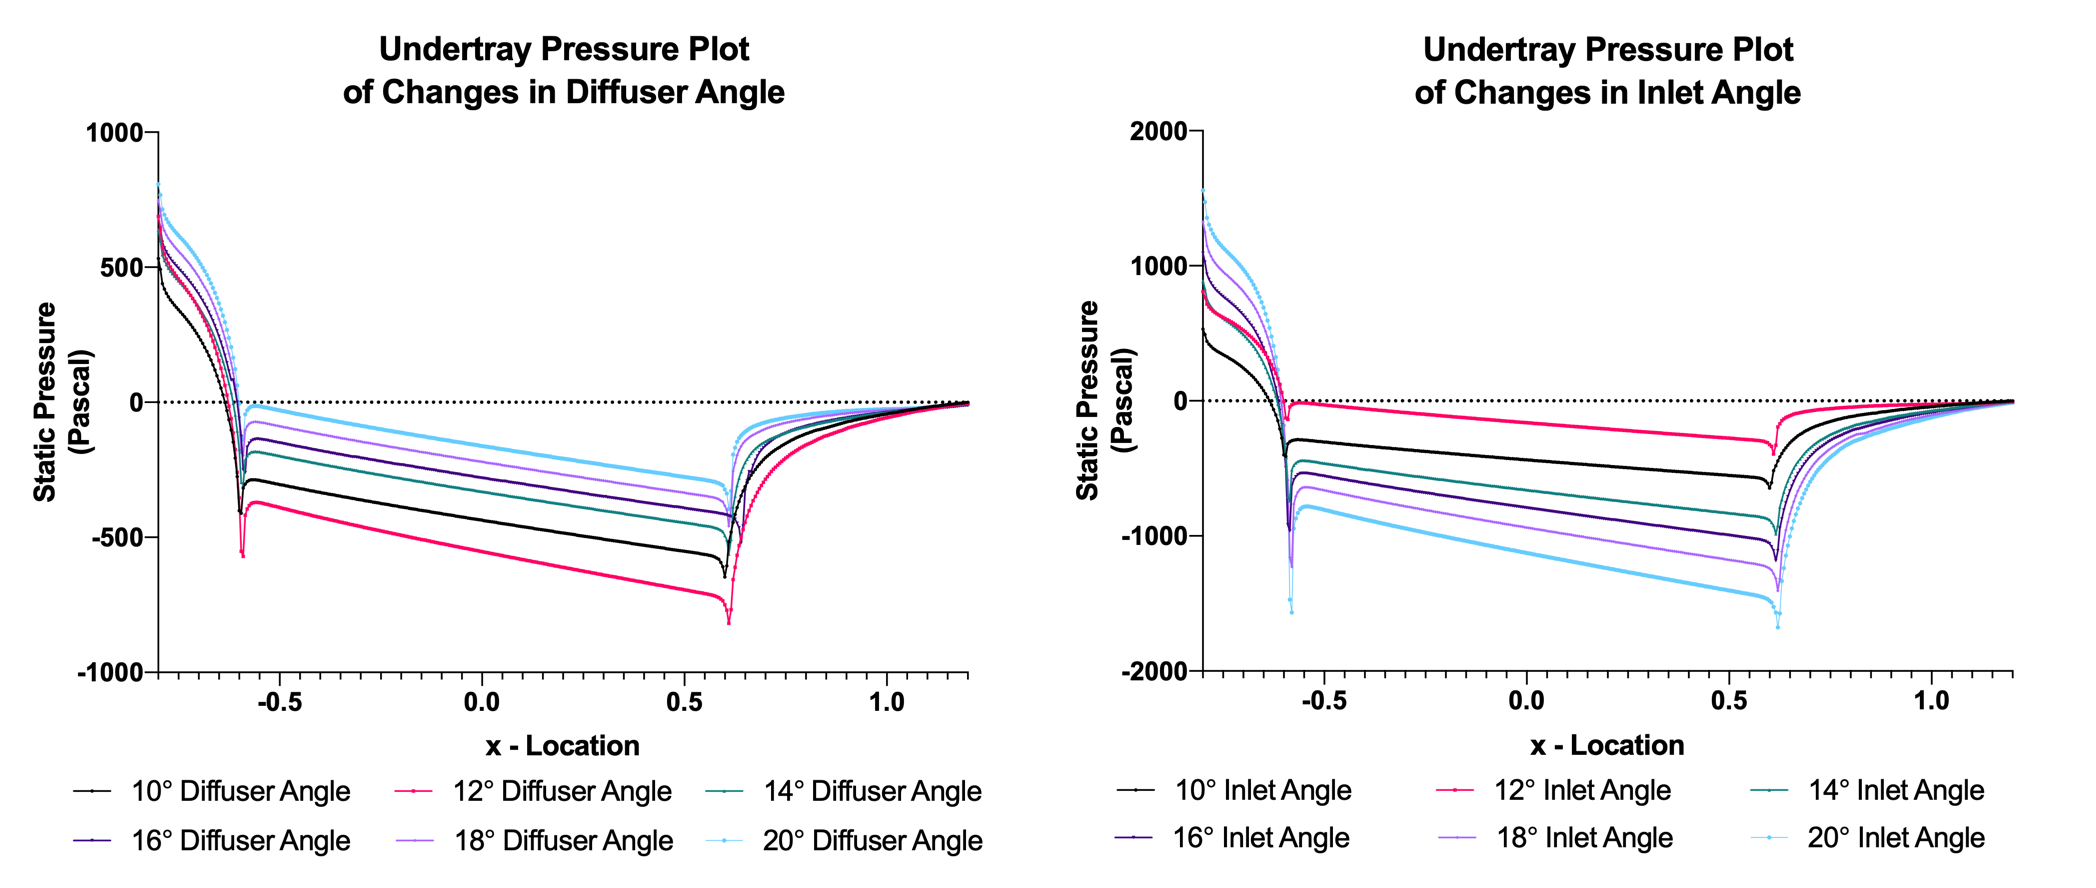
\includegraphics[width=1.1\textwidth]{Figures/2D_EN/2D_EN_UT_Presspdf.png}}
    \caption{Static Pressure Plot of Undertray's Wall With Changes in Diffuser (left) and Inlet (right) Angle.}
    \label{fig:pressure_plot_2D_EN}
\end{figure}

\begin{figure}
    \noindent\makebox[\textwidth]{
    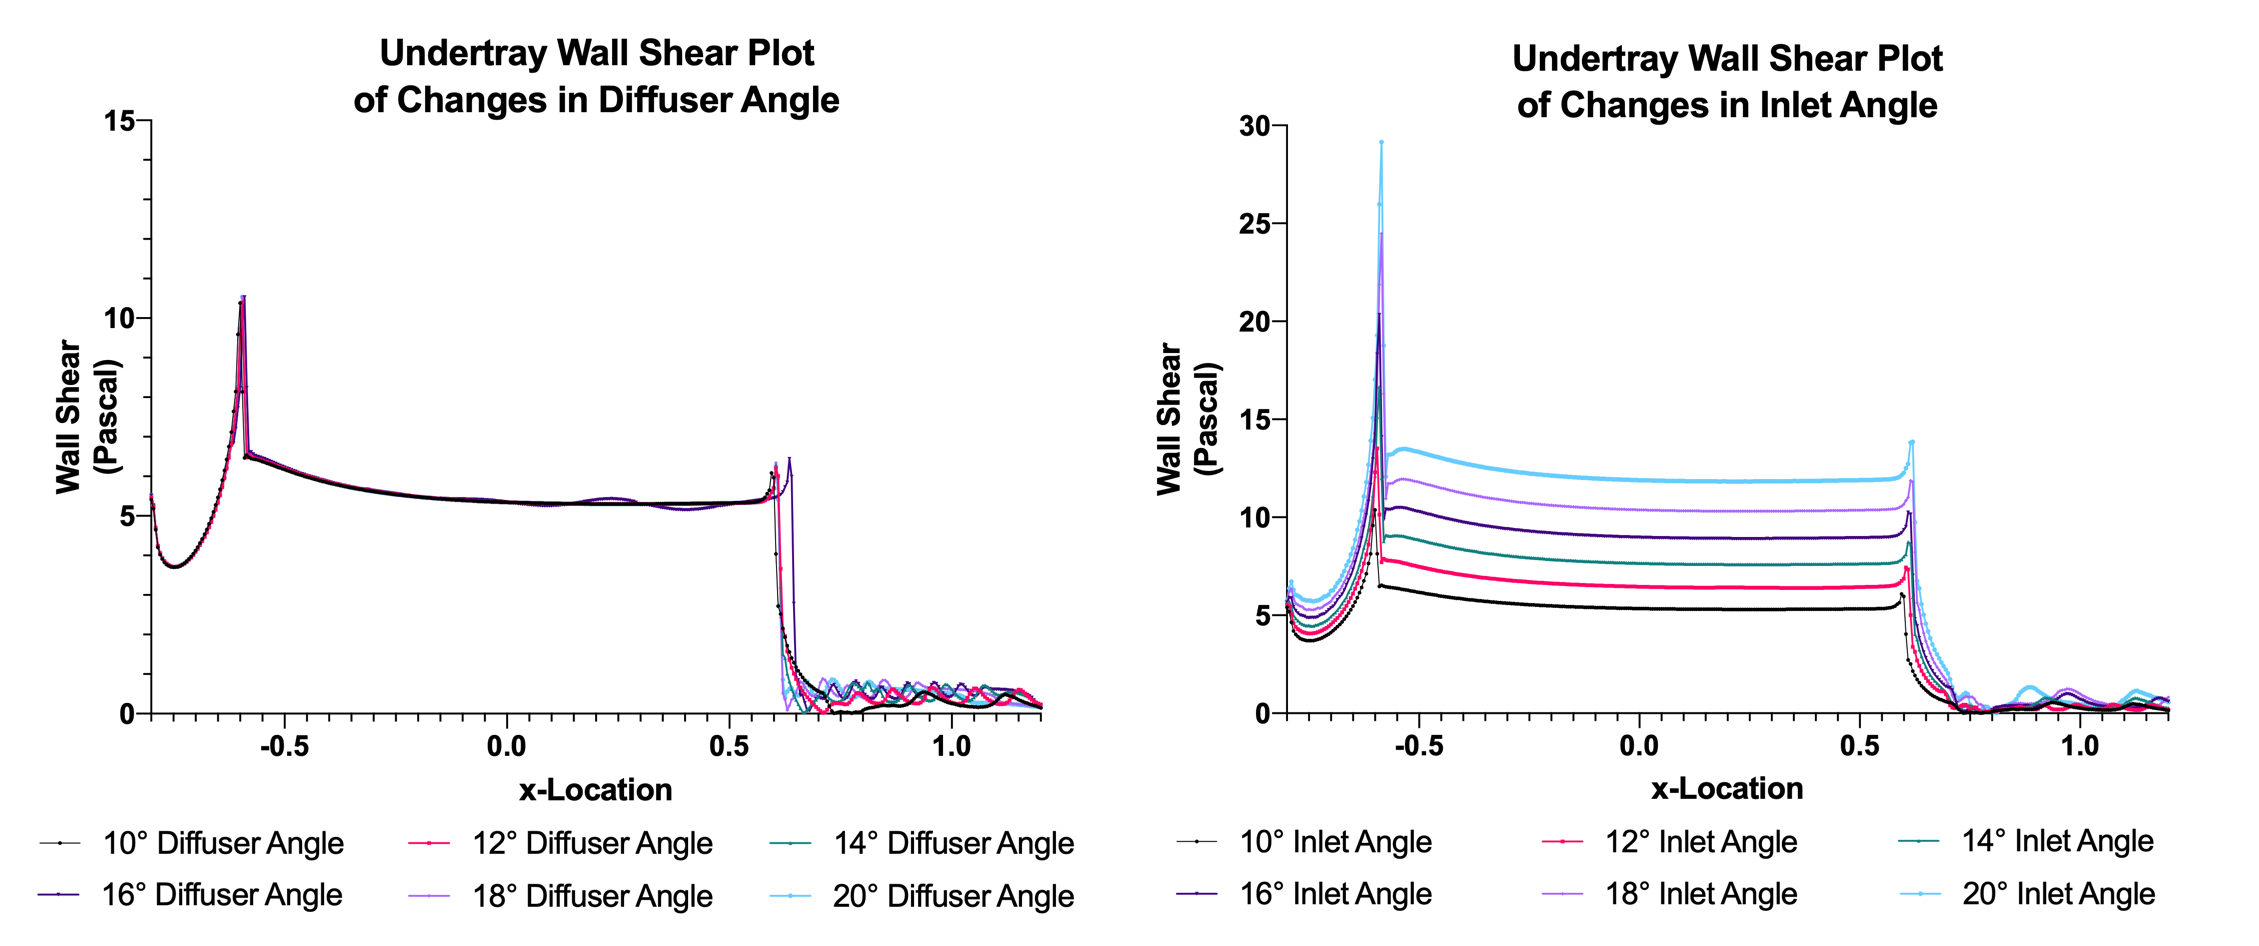
\includegraphics[width=1.1\textwidth]{Figures/2D_EN/2D_EN_UT_WShear.png}}
    \caption{$x$ Wall-Shear Plot of Undertray's Wall With Changes in Diffuser (left) and Inlet (right) Angle.}
    \label{fig:wall_shear_plot_2D_EN}
\end{figure}  
\end{center}


